\newif\ifinria
\def\ptitle{Recoloring graphs with Kempe changes} % Title
\def\pauthor{Clément Legrand-Duchesne} % Author
\def\padvisors{Marthe Bonamy, Vincent Delecroix} % Advisors
\def\pteam{Graphe et Optimisation, Combinatoire et Interactions} % Team
\def\pinstitute{Univ. Bordeaux, LaBRI, France} % Affiliation
\def\pdate{Thursday April 6, 2023} % Date
\inriafalse % inriatrue/inriafalse to enable/disable Inria logo


\pdfobjcompresslevel=0
\documentclass[final,hyperref={pdfpagelabels=false},xcolor=dvipsnames]{beamer}
\usepackage[orientation=portrait,size=a0,scale=1.4]{beamerposter}
\usepackage[utf8]{inputenc}
\usepackage[sfdefault]{roboto}
\usepackage[english]{babel}
\usepackage{amsmath, amsthm, amssymb, array, booktabs, grffile, latexsym, tabularx, xspace}
\newcolumntype{Z}{>{\centering\arraybackslash}X}
\newcommand{\pphantom}{\textcolor{ta3aluminium}}
\newlength{\columnheight}

\def\plogo{logo/logo_LaBRI.png}
\def\purl{https://www.labri.fr/}
\def\pmail{Twitter: @labriOfficial}

\mode<presentation>{\usetheme{SDSLaBRI}}
\title[\ptitle]{\texorpdfstring{\huge \ptitle}{\ptitle}}
\author[\pauthor]{\pauthor\ -\ \padvisors}
\institute[\pinstitute]{\pteam\ -\ \pinstitute}
\date[\pdate]{\pdate}
\setlogo{\plogo}
\setauthorurl{\purl}
\setauthoremail{\pmail}


\graphicspath{{./fig/}} % Figures and logos directory
\setlength{\columnheight}{588ex} % Tweak this value if columns are too long/short (should be okay with 588ex)

\usepackage{BeamerColor}
\usepackage{tikz}

%%%%%%%%% Colors of Beamer Layout %%%%%%%%%%%%%
\begin{document}
\begin{frame}
\begin{columns}
\begin{column}{.49\textwidth}
\begin{beamercolorbox}[center,wd=\textwidth]{postercolumn}
\begin{minipage}[T]{.95\textwidth}
\parbox[t][\columnheight]{\textwidth}{

\begin{block}{Graph coloring}
\begin{columns}
\begin{column}{.49\textwidth}

  \centering
  \pgfdeclarelayer{background}
  \pgfdeclarelayer{foreground}
  \pgfsetlayers{background,main,foreground}
  \begin{tikzpicture}

  \begin{pgfonlayer}{background} 
  \clip (-5,5) rectangle (5,-5);
  \draw[fill=yellow]  (0,0) -- (126:10cm) -- (198:10cm) -- cycle; 
  \draw[fill=rougeLaBRI]  (0,0) -- (198:10cm) -- (270:10cm) -- cycle;
  \draw[fill=bleuLaBRI]  (0,0) -- (270:10cm) -- (342:10cm) -- cycle;
  \draw[fill=yellow]  (0,0) -- (342:10cm) -- (54:10cm) -- cycle;
  \draw[fill=orange]  (0,0) -- (54:10cm) -- (126:10cm) -- cycle;
  \end{pgfonlayer}

  \begin{scope}[shift={(0,.75)}]
  \draw[fill=bleuLaBRI] (0,0) -- (45:3cm) -- (135:3cm) -- (0,0); 
  \draw[fill=orange] (0,0) -- (135:3cm) -- (225:3cm)-- (-90:2.12cm) -- (0,0); 
  \draw[fill=rougeLaBRI] (0,0) -- (-90:2.12cm) -- (315:3cm) -- (45:3cm) -- (0,0); 
  \end{scope}
  
  \begin{pgfonlayer}{foreground}
  \draw[fill=yellow] (0,-1.37) circle (1cm);
  \end{pgfonlayer}
  \end{tikzpicture}
  \end{column}
  \begin{column}{.49\textwidth}

  \centering
  \begin{tikzpicture}    
  \clip (-5,5) rectangle (5,-5);
  \node[draw=black,fill=orange,circle,inner sep=5pt]   (a) at (90:4cm) {};
  \node[draw=black,fill=yellow,circle,inner sep=5pt]  (b) at (162:4cm) {};
  \node[draw=black,fill=rougeLaBRI,circle,inner sep=5pt] (c) at (234:4cm) {};
  \node[draw=black,fill=bleuLaBRI,circle,inner sep=5pt] (d) at (306:4cm) {};
  \node[draw=black,fill=yellow,circle,inner sep=5pt] (e) at (18:4cm) {};

  \node[draw=black,fill=bleuLaBRI,circle,inner sep=5pt]   (f) at (90:1.7cm) {};
  \node[draw=black,fill=orange,circle,inner sep=5pt]  (g) at (180:1.7cm) {};
  \node[draw=black,fill=yellow,circle,inner sep=5pt] (h) at (270:1.7cm) {};
  \node[draw=black,fill=rougeLaBRI,circle,inner sep=5pt] (i) at (0:1.7cm) {};

  \draw (a) -- (b) -- (c) -- (d) -- (e) -- (a);
  \draw (f) -- (a)  (g) -- (b)  (i) -- (e);
  \draw (g) -- (i) -- (d) -- (h) -- (c) -- (g) -- (f) -- (i) -- (h) -- (g);
  \end{tikzpicture}
  \end{column}
  \end{columns}
  \vspace{1cm}
  [Apple, Haken 1989] Every planar map (or graph) is 4-colorable
\end{block}
            
            \vfill
            
            \begin{block}{Kempe change}
            
            \centering
  \begin{columns}
  \begin{column}{.49\textwidth}
  \centering
  \begin{tikzpicture}    
  \clip (-5,5) rectangle (5,-5);
  \node[draw=black,fill=orange,circle,inner sep=5pt]   (a) at (90:4cm) {};
  \node[draw=black,fill=yellow,circle,inner sep=5pt]  (b) at (162:4cm) {};
  \node[draw=black,fill=rougeLaBRI,circle,inner sep=5pt] (c) at (234:4cm) {};
  \node[draw=black,fill=bleuLaBRI,circle,inner sep=5pt] (d) at (306:4cm) {};
  \node[draw=black,fill=yellow,circle,inner sep=5pt] (e) at (18:4cm) {};

  \node[draw=black,line width = 3pt,fill=yellow,circle,inner sep=5pt]   (f) at (90:1.7cm) {};
  \node[draw=black,fill=orange,circle,inner sep=5pt]  (g) at (180:1.7cm) {};
  \node[draw=black,fill=yellow,circle,inner sep=5pt] (h) at (270:1.7cm) {};
  \node[draw=black,fill=rougeLaBRI,circle,inner sep=5pt] (i) at (0:1.7cm) {};

  \draw (a) -- (b) -- (c) -- (d) -- (e) -- (a);
  \draw (f) -- (a)  (g) -- (b)  (i) -- (e);
  \draw (g) -- (i) -- (d) -- (h) -- (c) -- (g) -- (f) -- (i) -- (h) -- (g);
  \end{tikzpicture}
  \end{column}
  
  \begin{column}{.49\textwidth}
  \centering
  \begin{tikzpicture}    
  \clip (-5,5) rectangle (5,-5);
  \node[draw=black,fill=orange,circle,inner sep=5pt]   (a) at (90:4cm) {};
  \node[draw=black,fill=yellow,circle,inner sep=5pt]  (b) at (162:4cm) {};
  \node[draw=black,line width = 3pt, fill=orange,circle,inner sep=5pt] (c) at (234:4cm) {};
  \node[draw=black,fill=bleuLaBRI,circle,inner sep=5pt] (d) at (306:4cm) {};
  \node[draw=black,fill=yellow,circle,inner sep=5pt] (e) at (18:4cm) {};

  \node[draw=black,fill=bleuLaBRI,circle,inner sep=5pt]   (f) at (90:1.7cm) {};
  \node[draw=black,line width = 3pt, fill=rougeLaBRI,circle,inner sep=5pt]  (g) at (180:1.7cm) {};
  \node[draw=black,fill=yellow,circle,inner sep=5pt] (h) at (270:1.7cm) {};
  \node[draw=black,line width = 3pt, fill=orange,circle,inner sep=5pt] (i) at (0:1.7cm) {};

  \draw (a) -- (b) -- (c) -- (d) -- (e) -- (a);
  \draw (f) -- (a)  (g) -- (b)  (i) -- (e);
  \draw  (i) -- (d) -- (h) -- (c)  (g) -- (f) -- (i) -- (h) -- (g);
  \draw[line width = 3pt] (c) -- (g) -- (i);
  \end{tikzpicture}
  \end{column}
  \end{columns}
  \vspace{1cm}
  Kempe change: swap the colors in a maximal bichromatic connected subgraph
            
            \end{block}
            
            \vfill
            
            \begin{block}{Objectives and questions}
            
            \centering
            \begin{itemize}
            \item Color a graph with as few colors as possible
            \item 
            \item 
            \end{itemize}
            \end{block}
            
            \vfill
            
            \begin{block}{MS-Stream: Multi-Source Streaming over HTTP}
            
            \centering
            
            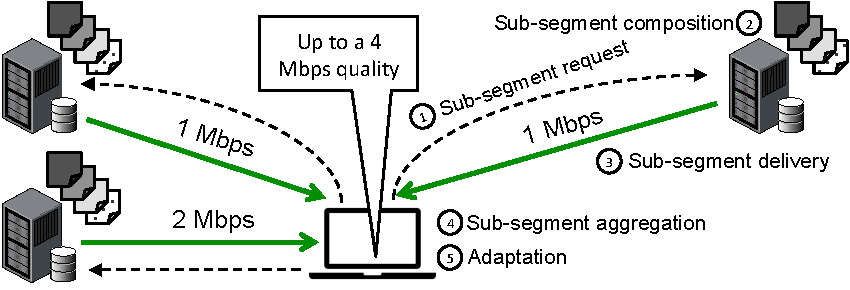
\includegraphics[width=.925\textwidth]{sample/msstream_archi.pdf}
            
            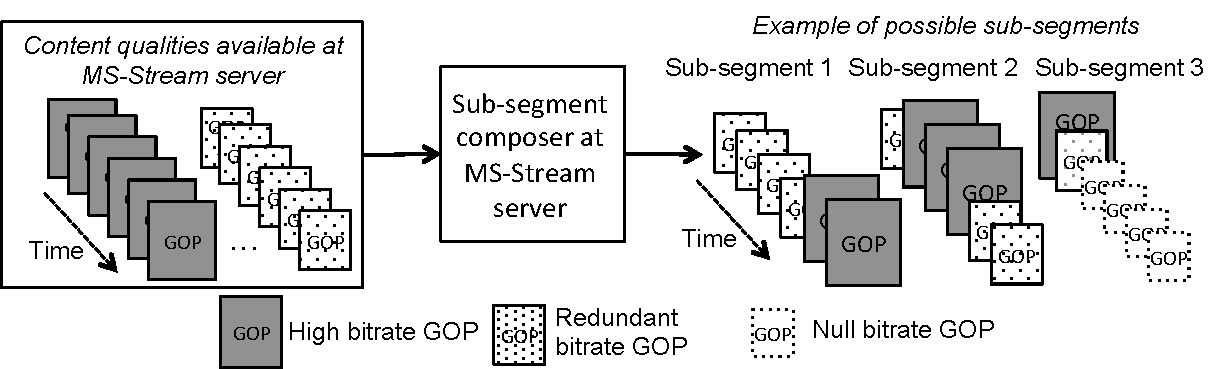
\includegraphics[width=.925\textwidth]{sample/chunk2.pdf}
            
            \end{block}
            
            \vfill
            
            \begin{block}{Problem statement}
            
            \centering
            
            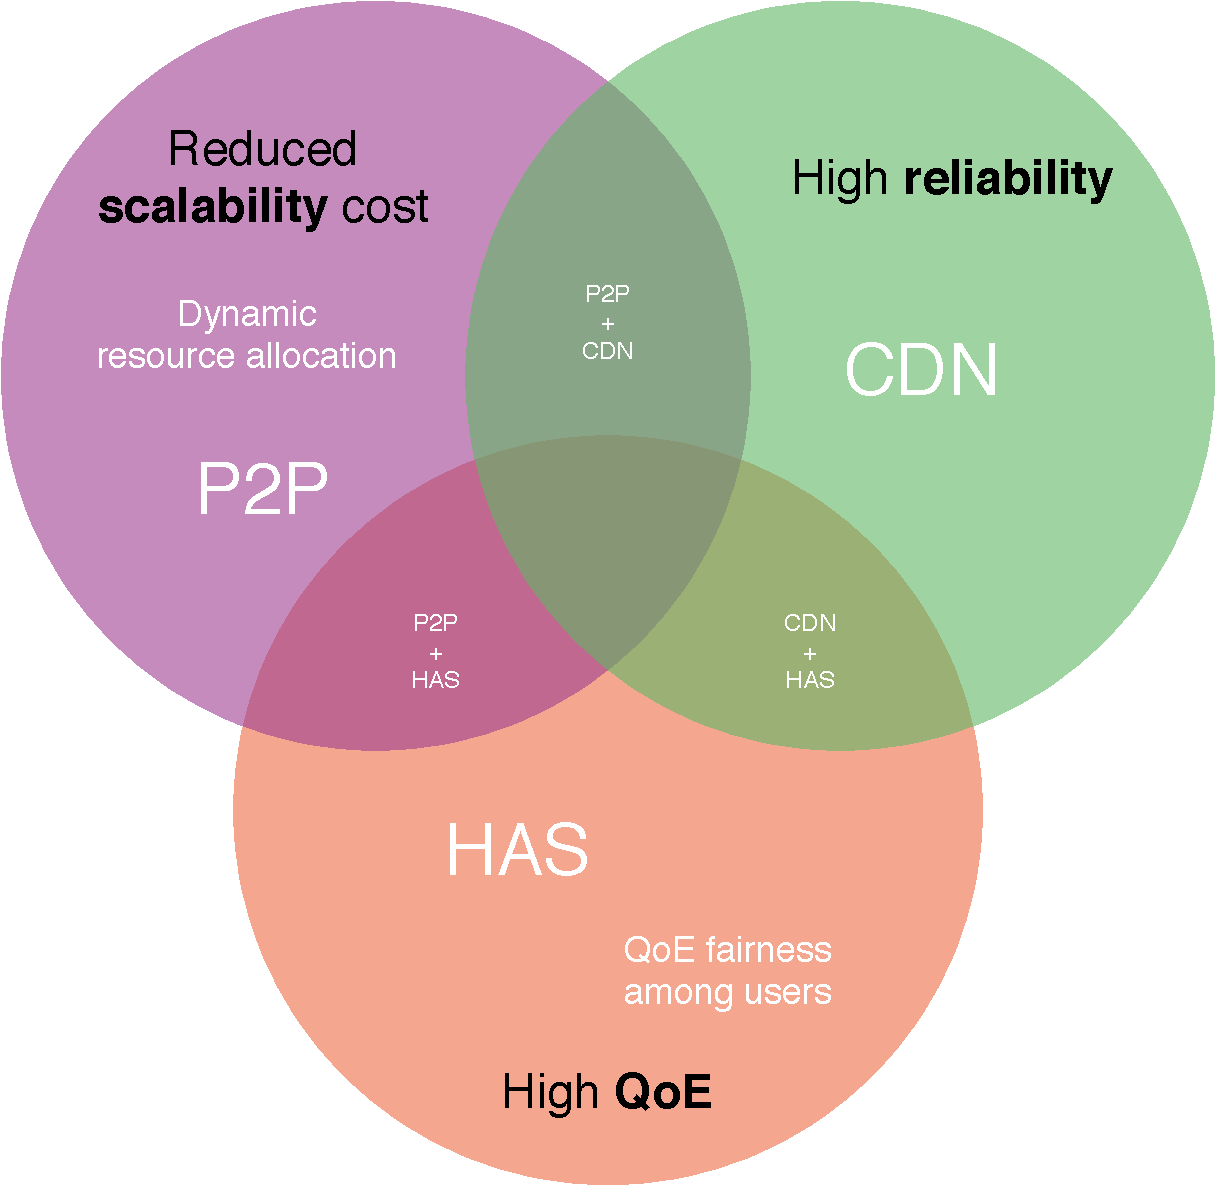
\includegraphics[width=.5\textwidth]{sample/SotA-cropped.pdf}
            
            \end{block}
            
          }
        \end{minipage}
      \end{beamercolorbox}
    \end{column}
    \begin{column}{.49\textwidth}
      \begin{beamercolorbox}[center,wd=\textwidth]{postercolumn}
        \begin{minipage}[T]{.95\textwidth}
          \parbox[t][\columnheight]{\textwidth}{
            
            \begin{block}{ idea}
            
            \begin{itemize}
            
            \item Reliability, QoE and scalability
            
            MS-Stream: Multiple-Source adaptive streaming over HTTP
            
            \item Incentive to contribute
            
            Rewarding: contributing users get a higher quality
            
            \item End-users privacy
            
            TEE (SGX): encryption, NAT and anonymity
            
            \end{itemize}
            
            \end{block}
            
            \vfill
            
            \begin{block}{ overview}
            
            \centering
            
            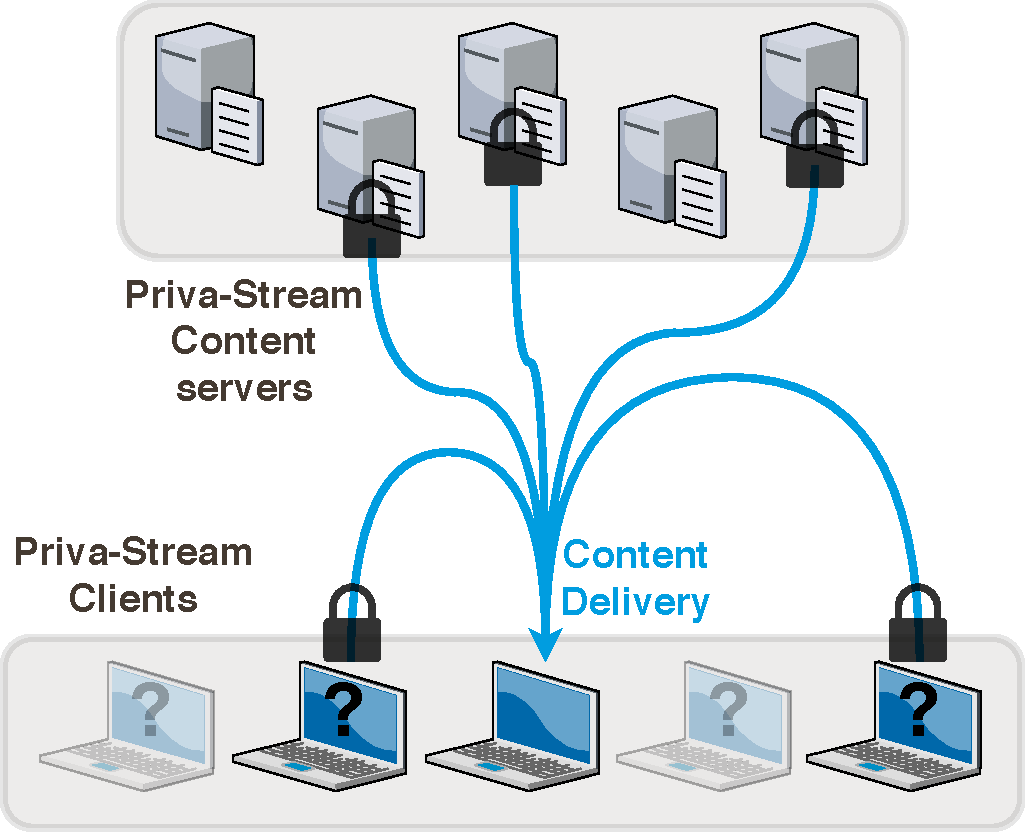
\includegraphics[width=.925\textwidth]{sample/BP.pdf}
            
            \end{block}
            
            \vfill
            
            \begin{block}{ technical description}
            
            \centering
            
            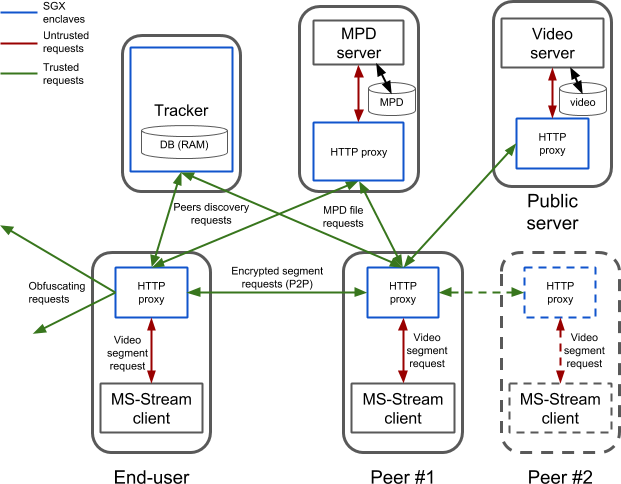
\includegraphics[width=.8\textwidth]{sample/PS-tech.png}
            
            \end{block}
            
            \vfill
            
            \begin{block}{ early results}
            
            \centering
            
            Experiment: Four clients joining the system sequentially
            
            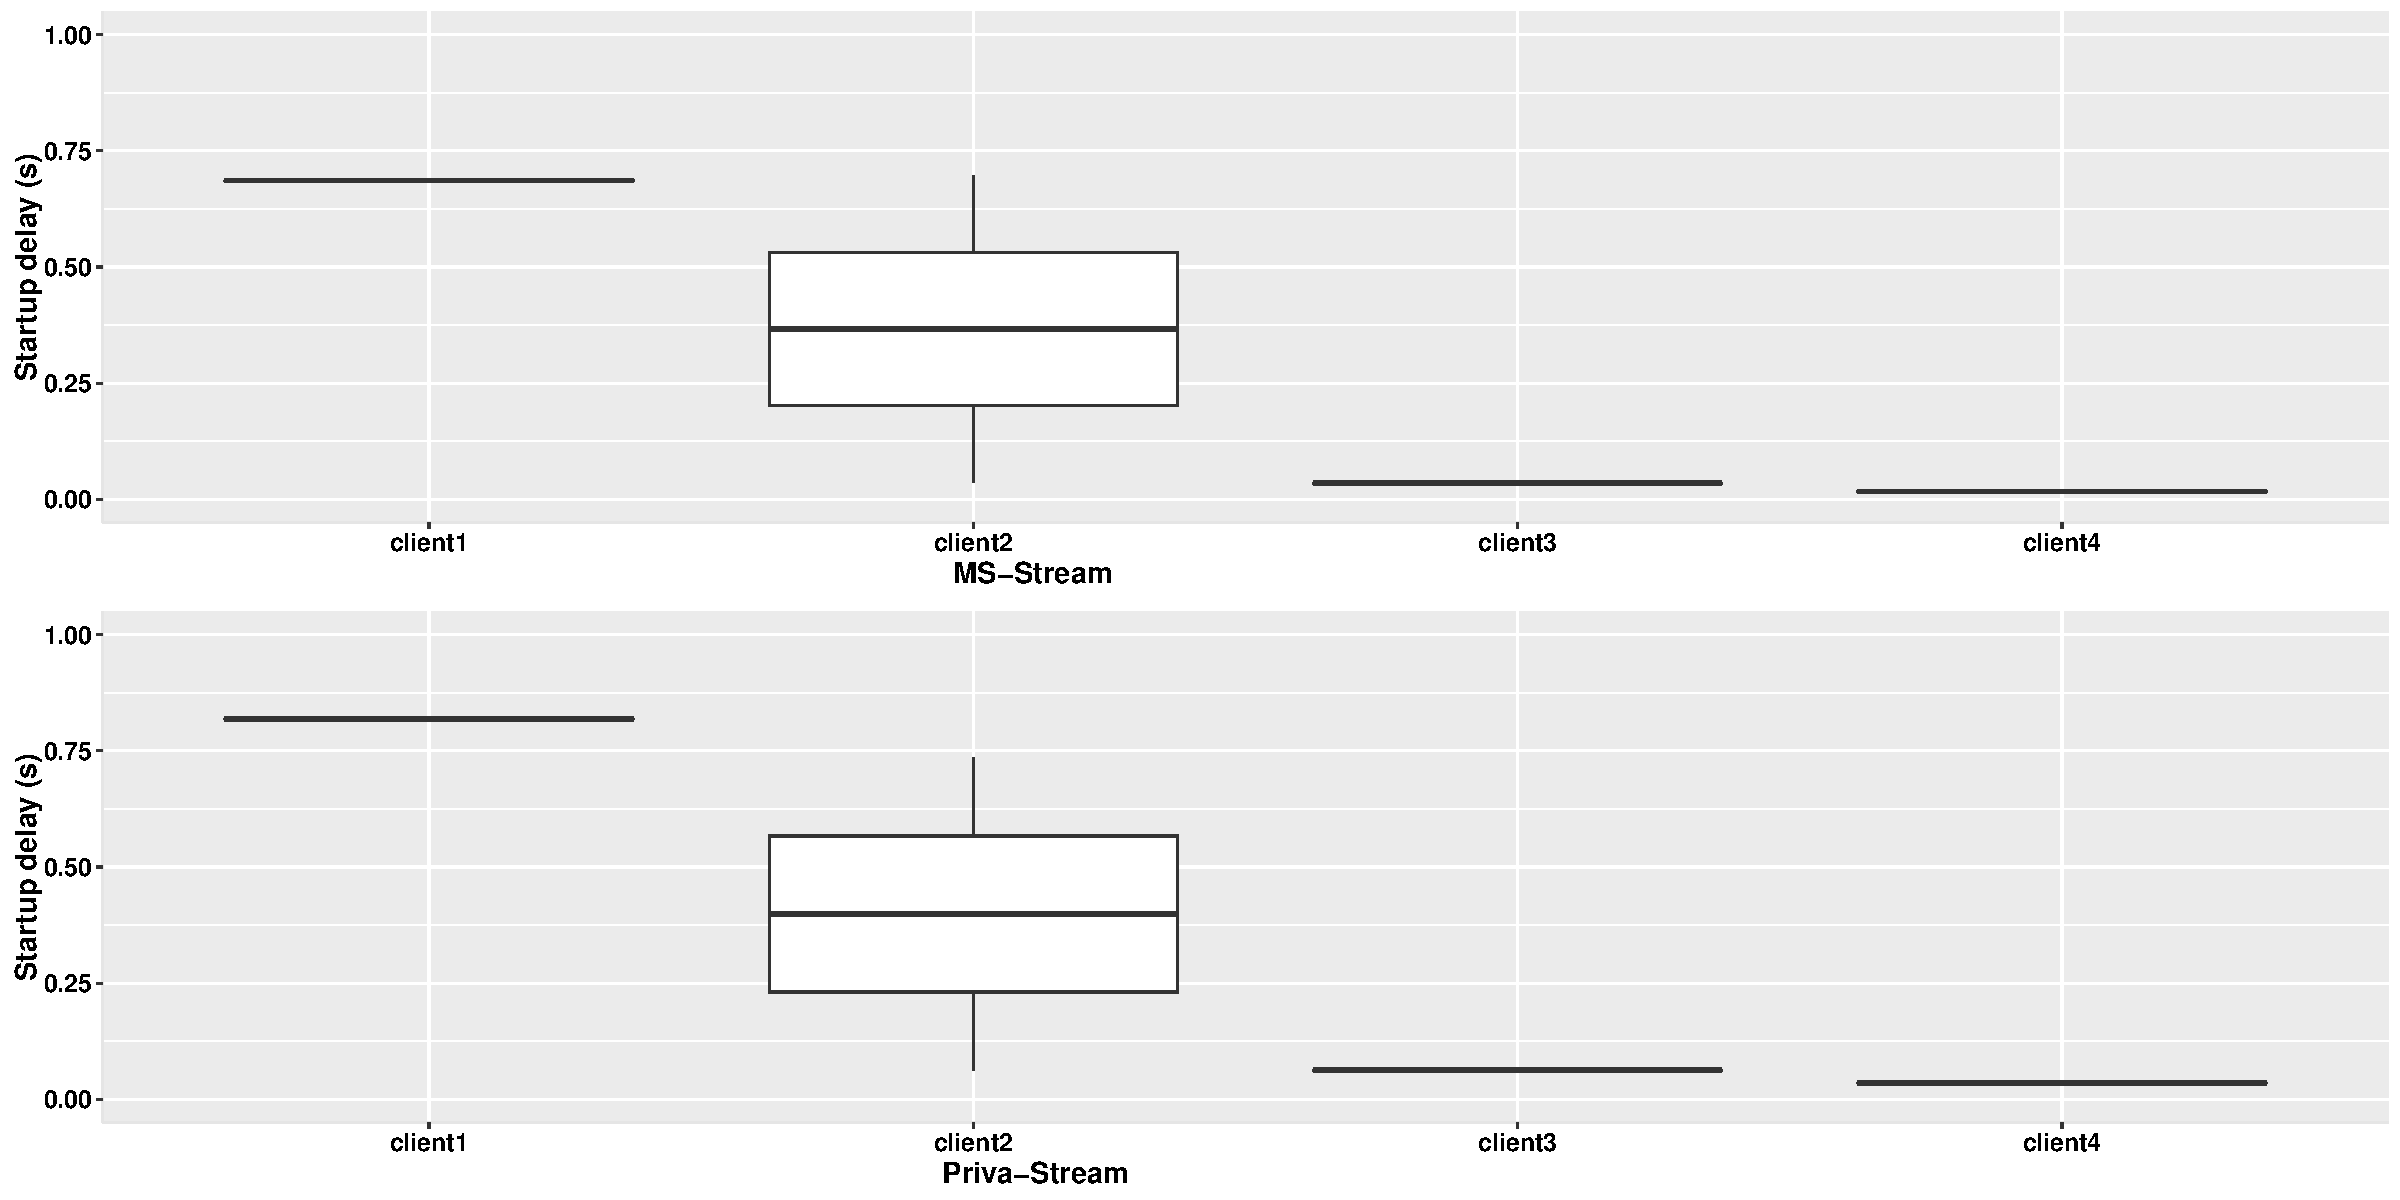
\includegraphics[width=.925\textwidth]{sample/startup.pdf}
            
            Startup delay (s) - MS-Stream (top) vs (bottom)
            
            \end{block}
            
          }
        \end{minipage}
      \end{beamercolorbox}
    \end{column}
  \end{columns}
  \vskip1ex
\end{frame}
\end{document}
